\documentclass[11pt]{article}






%\usepackage{times}
\usepackage{palatino}%charter}
\usepackage{multirow}
\usepackage{wrapfig}
\usepackage{url}
\usepackage{citesort}
\usepackage{epsfig}
\usepackage{graphicx}
\usepackage{color}
\usepackage{fullpage}
\usepackage{amssymb}
\usepackage{amsmath}
\usepackage{theorem}
%\theoremstyle{remark} 
%\theoremstyle{definition}
%\usepackage{wide}
%\usepackage[ruled, vlined]{algorithm2e}
\usepackage[ruled, vlined, linesnumbered]{algorithm2e}
\usepackage{color}
%\usepackage{hyperref}
\usepackage{subfig}
\usepackage{pgf}
\usepackage[a4paper,top=10.0mm,bottom=15.0mm]{geometry}

\newcommand{\veps}{\varepsilon}
\newcommand{\eps}{\epsilon}
\newcommand{\E}{\mathbf{E}}
\renewcommand{\Pr}{\mathbf{Pr}}
\newcommand{\abs}[1]{\left| #1 \right|}
\newcommand{\norm}[1]{\left\lVert #1 \right\rVert}

\newcommand{\bbR}{\mathbb{R}}
\newcommand{\bbZ}{\mathbb{Z}}
\newcommand{\calC}{\mathcal{C}}
\newcommand{\calI}{\mathcal{I}}
\newcommand{\calM}{\mathcal{M}}
\newcommand{\calK}{\mathcal{K}}
\newcommand{\emRed}[1][]{\textcolor{blue} #1}
\newcommand{\opt}{\text{OPT}}
\newcommand{\knowopt}{{\sc KnowOpt}}
\newcommand{\alg}{\text{ALG}}
\newcommand{\greedy}{{\sc Greedy}~}
\newcommand{\greedyLazy}{{\sc GreedyLazy}~}
\newcommand{\stocGreedy}{{\sc StocGreedy}~}
%\newcommand{\baseline}{{\sc BaselineStream}~}
\newcommand{\randomSampling}{{\sc RandomSampling}~}
\newcommand{\sieveStream}{{\sc SieveStream}~}
\newcommand{\randomStream}{{\sc RandomStream}~}
\newcommand{\circuitStream}{{\sc CircuitStream}~}
\newcommand{\offline}{{\sc Offline}~}

\newtheorem{theorem}{Theorem}
\newtheorem{protocol}{Protocol}
\newtheorem{lemma}{Lemma}
\newtheorem{claim}{Claim}
\newtheorem{property}{Property}
\newtheorem{fact}{Fact}
\newtheorem{observation}{Observation}
\newtheorem{heuristic}{Heuristic}
\newtheorem{solution}{Solution}
\newtheorem{corollary}{Corollary}
\newtheorem{scheme}{Scheme}
\newtheorem{strategy}{Strategy}
\newtheorem{invariant}{Invariant}
{\theorembodyfont{\rmfamily}
\newtheorem{remark}{Remark}}
{\theorembodyfont{\rmfamily}
\newtheorem{definition}{Definition}}

\DeclareMathOperator*{\argmin}{arg\,min}
\DeclareMathOperator*{\argmax}{arg\,max}


\newcommand{\chensays}[2][]{\textcolor{red} {\textsc{Chen #1:} \emph{#2}}}




\newenvironment{proof}{\trivlist\item[]\emph{Proof:}}%
{\unskip\nobreak\hskip 1em plus 1fil\nobreak$\Box$
\parfillskip=0pt%
\endtrivlist}





\begin{document}

\title{Report: Experimental Study for Submodular Maximization}
\author{Jiecao Chen\\ jiecchen@indiana.edu}
\date{\today}

\maketitle



%----------- start -----------------------
k\section{Roadmap}
In this part, we give an experimental study of submodular maximization. In Section \ref{sec:setup} we cover the setup for our experiment; we then compare three greedy algorithms in Section \ref{sec:greedy}; In Section \ref{sec:streaming} we compare three streaming algorithms with random sampling and the offline greedy algorithm; we discuss {\sc GreeDi}-based distributed algorithms in Section \ref{sec:distributed} and conclude this report in Section \ref{sec:conclude}.

\section{The Setup}
\label{sec:setup}

\subsection{Submodular Functions}
We mainly consider two type of submodular functions in our experiment.
\paragraph{Set Cover Problem}
In the \emph{set cover problem}, we are given a collection of subsets of a set $E$, i.e. $V = \{C_1, C_2, \ldots, C_n\}$ where each $C_i \subseteq E$. We define a function $f:2^V \rightarrow \bbR$ such that $f(S) = |\cup_{C\in S} C|$. We can interpret $f$ as follow: given $S$ as a subset of $V$, the value of $f(S)$ is the number of distinct elements covered by the sets in $S$.

One can easily verify that $f$ satisfies the diminishing return property thus is a submodular function. Furthermore, it is clear that $f$ is non-decreasing.  Now given the cardinality constraint, we want to solve the following,

$$\argmax_{S\subseteq V: |S|\leq k} f(S).$$

\paragraph{Weighted Vertex Function}
Let $G = (V, E, W)$ be a graph where each $v\in V$ has a weight $w_v > 0$. For any $S \subseteq E$, $V(E)$ is the set of vertices of edges in $S$. Let $f: 2^E \rightarrow \bbR$ be a set function with $f(S) =\sum_{v\in V(S)} w_{v}$, then $f$ is submodular. We call $f$ a \emph{weighted vertex function}.



% \subsection{Informative Vector Machine}
% Kernel machines \cite{SS02} are powerful non-parametric learning techniques. Those approaches use kernel trick to reduce non-linear problems to linear tasks that have been well studied. The data set $V = \{x_1, x_2, \ldots, x_n\}$ is represented in a transformed space via a kernel matrix

% \[ K_V = \left( \begin{array}{ccc}
% \calK(x_1, x_2) & \ldots & \calK(x_1, x_n) \\
% \vdots & \ddots & \vdots \\
% \calK(x_n,x_1) & \ldots & \calK(x_n, x_n) \end{array} \right)\] 
% here $\calK: V\times V \rightarrow \bbR$ is the kernel function that is symmetric and positive definite. 

% For large-scale problem, even representing the matrix $K_V$ (which requires $O(n^2)$ space) is prohibited. The common solution to solve this issue is to select a small representative subset $S \subseteq V$ and only work with $K_S$. The question now becomes how to select the subset $S$. One popular way to measure the quality of selected set $S$ is to use \emph{Informative Vector Machine}(IVM) introduced by Laurence et al. \cite{LSH03}. Formally, we define $f: 2^V \rightarrow \bbR$ with
% $$f(S) = \frac{1}{2} \log\det\left( \mathbf{I} + \sigma^{-2} K_S \right)$$
% where $\mathbf{I}$ is the identity matrix and $\sigma > 0$ is a parameter. IVM has a close connection to the entropy of  muti-variable Gaussian distribution \cite{B14} and it is shown in \cite{S04,B14} that $f$ is a submodular function. We can then select the set $S\subset V$ by solving
% $$\argmax_{S:|S|\leq k} f(S).$$

% In our experiment, we use the heat kernel $\calK_h(e1, e2) = \exp\{-\|e_1-e_2\|_2^2/h^2\}$ where $h > 0$ is a parameter.


\subsection{Datasets}
\paragraph{Synthetic:} We create $1000$ subsets of $[1000] = \{1, 2, \ldots, 1000\}$ , each subset is randomly constructed as follows: 1) randomly sample an integer $n$ from $[1, 100)$ as the size; 2) randomly sample $n$ elements without replacement from $[1000]$. The {\sc Synthetic } dataset is then a collection of $1000$ sets.


\paragraph{Facebook:} 
The {\sc Facebook} dataset is a friends list collected from Facebook users. This dataset is an undirected graph with $4039$ nodes, $88234$ edges. More information of this dataset can be found in \cite{snapnets} ego-Facebook.  We assign each node its degree as its weight. The original edges are grouped by nodes.

\paragraph{Accidents:} dataset is publicly available from \url{http://fimi.ua.ac.be/data/}. Each line of {\sc Accidents} can be considered as a subset of $[n]$ for a fixed $n$. The original dataset has $340,183$ subsets. Due to lack of computation resources, we only take the first $10,000$ subsets in our experiment. More information of this dataset can be found in \url{http://fimi.ua.ac.be/data/accidents.pdf}. 

\subsection{Computation Environments}
Due to lack of computation resources, all experiments were run in a personal laptop with $3.7$GB Memory, $119$GB SSD, 1.70GHzx2-Intel Core i5 CPU. The operating system is Linux Mint 7.2 Cinnamon 64-bit. 

\subsection{Code} 
Most code for this experiment is available at 
\begin{itemize}
\item \url{https://github.com/jiecchen/SubmodularLib/tree/master/src}~.
\end{itemize}
It contains about $3000$ lines of java and python code.

\subsection{Comments on Randomized Algorithms}
For randomized algorithms, we run experiments for about $10$ times; the results are then presented as error bar with $2\sigma$,  which is $95\%$ confidence interval. 

\section{Simple Greedy Algorithms}
\label{sec:greedy}
In this section, we compare three different greedy algorithms in the problem of monotone submodular maximization subject to cardinality constraint. We compare their efficiency (measured by number of value queries) and the quality of solutions they returned.
\subsection{Greedy Algorithms}
Let $V$ be the ground set and $k$ be the cardinality constraint. $ 0 < \eps < 1$ is a parameter to control the error.
\begin{itemize}
\item \greedy is the standard greedy algorithm that gives $(1 - e^{-1})$-approximation.  See Algorithm \ref{algo:greedy} for details.
\item \greedyLazy is the greedy algorithm with the trick of lazy evaluation \cite{M78}. The idea goes as follows: instead of computing $\Delta_f(e|S)$ for each $e\in V\backslash S$ in Line \ref{line:emax} of Algorithm \ref{algo:greedy},  \greedyLazy keeps an upper bound $\rho(e)$ (initially $+\infty$) on the marginal gain sorted in decreasing order (or kept in a heap). In each iteration, the \greedyLazy algorithm evaluates the element on top of the heap and updates its upper bound via $\rho(e) \gets \Delta(e|S)$. If the updated $\rho(e) \geq \rho(e')$ for all other $e'$, submodularity guarantees that $e$ is the element with the largest marginal gain. The \greedyLazy algorithm again gives $(1 - e^{-1})$-approximation.
\item \stocGreedy is a sampling-based greedy algorithm. In each step where we add one new element to the solution, we consider only a small fraction of the remaining elements ($O(\frac{|V|}{k}\log \frac{1}{\eps})$). In the selected portion of elements, we also use lazy evaluation to obtain further speedup. This algorithm gives $(1 - e^{-1} - \eps)$-approximation in expectation. We omit its detailed description.
\end{itemize}

\begin{algorithm}[H]
\DontPrintSemicolon % Some LaTeX compilers require you to use \dontprintsemicolon instead
\KwIn{$V$ the ground set, $f$ the submodular function, $k$ the cardinality constraint}
\KwOut{a set $S \subseteq V$}
$S \gets \emptyset$\;
\While{$|S| < k$} {
  $e \gets \argmax_{e\in V\backslash S} \Delta_f(e|S)$\;\label{line:emax}
  $S \gets S\cup \{e\}$\;
}
\Return{$S$}\;
\caption{\greedy for submodular maximization subject to cardinality constraint}
\label{algo:greedy}
\end{algorithm}

\subsection{Results for {\sc Synthetic}}
Figure \ref{fig:greedy-efficiency} shows that both \greedyLazy and \stocGreedy significantly outperform \greedy in terms of number of value queries being called. \stocGreedy is even faster than \greedyLazy.  Figure \ref{fig:quality-greedy} shows that \greedy, \greedyLazy and \stocGreedy return solutions with similar quality; \stocGreedy produces slightly worse solution compared with other two.

\begin{figure*}[h!t]
     \centering
     \subfloat[][Efficiency]{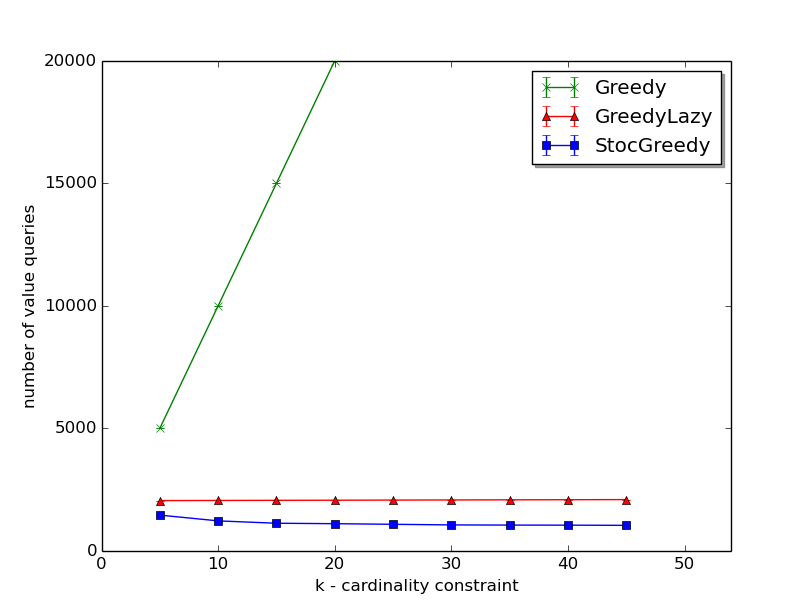
\includegraphics[width=0.5\textwidth]{figures/value-queries}\label{fig:greedy-efficiency}}
     ~~
     \subfloat[][Quality]{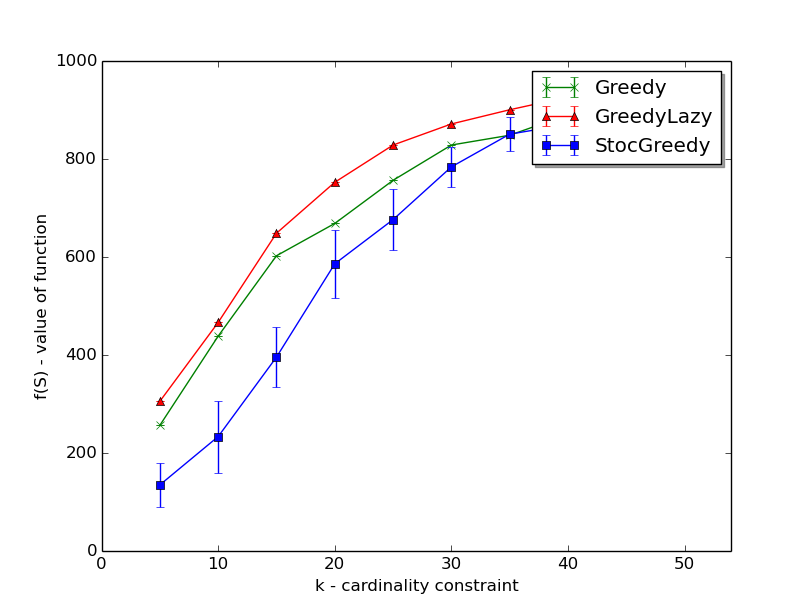
\includegraphics[width=0.5\textwidth]{figures/func-values}\label{fig:quality-greedy}}    
     \caption{Experiment on {\sc Synthetic} dataset}
     \label{fig:sythetic-offline}
\end{figure*}


% \begin{figure}[!ht]
%     \centering
%     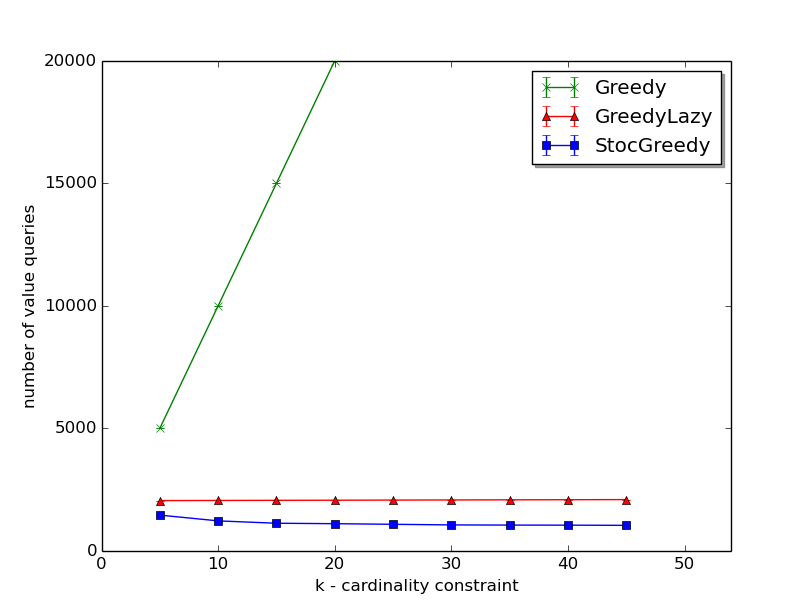
\includegraphics[width=0.5\textwidth]{figures/value-queries.png}
%     \caption{{\sc Synthetic}: efficiency, measured by number of value queries being used.}
%     \label{fig:greedy-efficiency}
% \end{figure}

% \begin{figure}[!ht]
%     \centering
%     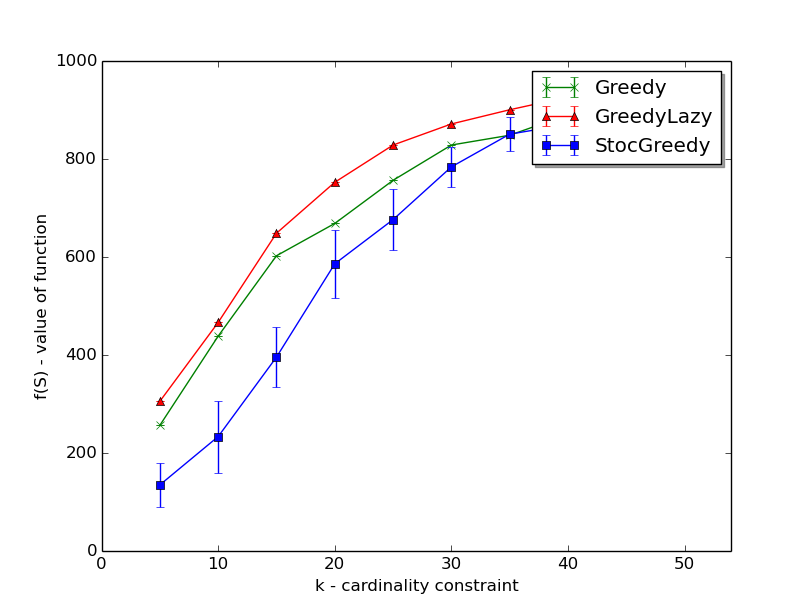
\includegraphics[width=0.5\textwidth]{figures/func-values.png}
%     \caption{{\sc Synthetic}: quality of returned solutions}
%     \label{fig:quality-greedy}
% \end{figure}



\section{Streaming Submodular Maximization}
\label{sec:streaming}
We compare three different streaming algorithms in the problem of monotone submodular maximization subject to cardinality constraint. In generally it is hard to compare those algorithms fairly because they are configured by different type of parameters. To address this issue, we fix parameters so that all three algorithms consume roughly the same amount of time. We also compare them with  the standard greedy algorithm (here we call it \offline) and a streaming algorithm (called \randomSampling) that generates the solution by using random sampling (the notable reservoir sampling is being used internally).


\subsection{Streaming Algorithms}
\begin{itemize}
\item \sieveStream \cite{BMK+14} gives $(1/2 - \eps)$-approximation. See \ref{algo:sieveStream} for details.
\item \randomStream \cite{CGQ15} gives $\frac{1 - \eps}{2 + \eps}$-approximation. See \ref{algo:randomStream} for details.
\item \circuitStream \cite{V11,CGQ15} gives $1/4$-approximation. See \ref{algo:circuitStream} for details.
\end{itemize}
We also compare above three algorithms with \offline and \randomSampling as mentioned.

\begin{algorithm}[H]
\DontPrintSemicolon % Some LaTeX compilers require you to use \dontprintsemicolon instead
\KwIn{$V$ as data stream, $f$ a monotone submodular function, $k$ the size constraint, $\eps$ a parameter}
\KwOut{a set $S \subseteq V$}
$O = \{(1 + \eps)^i~|~i\in \bbZ\}$\;
\tcc*[h]{maintain the sets only for the necessary $v$'s lazily}\;
For each $v\in O, ~S_v \gets \emptyset$\;
$m \gets 0$\;

\For{each $e$ in the data stream} {
  $m \gets \max\{m, f(\{e\})\}$\;
  $O\gets \{(1 + \eps)^i~|~m \leq (1 + \eps)^i \leq 2\cdot k \cdot m\}$\;
  Delete all $S_v$ such that $v \in O$\;
  \For{$v \in O$}{
    \If{$\Delta(e|S_v) \geq \frac{v/2 - f(S_v)}{k - |S_v|}$ and $|S_v|<k$}{
      $S_v \gets S_v \cup \{e\}$\;
    }
  }
}
\Return{$\argmax_{S_v: v\in O}f(S_v)$}\;
\caption{\sieveStream for submodular maximization}
\label{algo:sieveStream}
\end{algorithm}

\begin{algorithm}[H]
\DontPrintSemicolon % Some LaTeX compilers require you to use \dontprintsemicolon instead
\KwIn{$V$ as data stream, $f$ a non-negative submodular function, $k$ the cardinality constraint, $\eps$ a parameter}
\KwOut{a set $S \subseteq V$}
$B\gets \emptyset, S\gets \emptyset$\;
\For{each $e$ in the data stream} {
  \If{$|S| < k$ and $\Delta(e|S) > \alpha$}{
    $B \gets B + e$\;
  }
  \If{$|B| > \frac{k}{\eps}$}{
    $e \gets $ uniformly random from $B$\;
    $B \gets B - e, S \gets S + e$\;
    \For{all $e'\in B$ s.t. $\Delta(e'|S)\leq \alpha$}{
      $B \gets B - e'$\;
    }
  }
}
$S' \gets$ offline algorithm on $B$\;
\Return{$\argmax_{A\in\{S, S'\}}f(A)$}\;
\caption{\randomStream for submodular maximization}
\label{algo:randomStream}
\end{algorithm}

\begin{algorithm}[H]
\DontPrintSemicolon % Some LaTeX compilers require you to use \dontprintsemicolon instead
\KwIn{$V$ as data stream, $f$ a monotone submodular function, $k$ is the cardinality constraint, $\gamma > 0$ is a parameter}
\KwOut{a set $S \subseteq V$}

\For{each $e$ in the data stream} {
  \If{$|S| < k$}{
    $S \gets S + e$\;
  }
  \Else{
    $e^* \gets \argmin_{e'\in S}f(\{e'\})$\;       
    \If{$f(\{e\}) \geq (1 + \gamma)\cdot f(\{e^*\})$}{
      $S \gets S \cup \{e\} \backslash \{e^*\}$\;
    }  
  }
}
\Return $S$\;
\caption{\circuitStream for  submodular maximization}
\label{algo:circuitStream}
\end{algorithm}

\subsection{Results for {\sc Facebook}}
Figure \ref{fig:streaming-shuffle} shows the results of streaming algorithms that run on shuffled {\sc Facebook} dataset.  The results are interesting because \sieveStream and \randomStream can produce better solutions (measured by function value) than \offline. Part of the reason is that both \sieveStream and \randomStream run many copies of fixed-threshold streaming algorithms in parallel and latter pick the best among the solutions produced by those algorithms; it might be more likely to generate ``good'' solutions.  Perhaps somewhat surprising, the solution produced by \circuitStream is even worse than \randomSampling. The result of \circuitStream, however, does not violate the theoretical result (which only guarantees $1/4$-approximation); more experiments are required before we can explain this phenomenon.


Figure \ref{fig:streaming-not-shuffle} shows the results on non-shuffled {\sc Facebook} dataset where edges are grouped by vertices. As we can see from this figure, \offline is independent of  the order of input data due to the way it works (see Algorithm \ref{algo:greedy}); but the order does matter to streaming algorithms. In the non-shuffled dataset, \offline generates the best solution and the solution returned by \sieveStream is comparably good; \randomStream generates slightly worse result while  \circuitStream  again has the worse performance.



\begin{figure*}[h!]
     \centering
     \subfloat[][Shuffled edges]{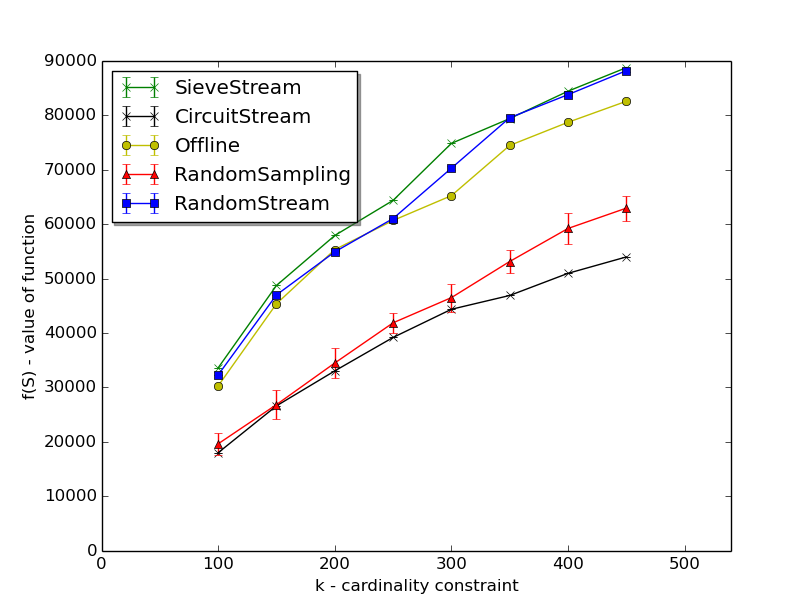
\includegraphics[width=0.5\textwidth]{figures/streaming-shuffle}\label{fig:streaming-shuffle}}
     ~~
     \subfloat[][Edges grouped by vertices]{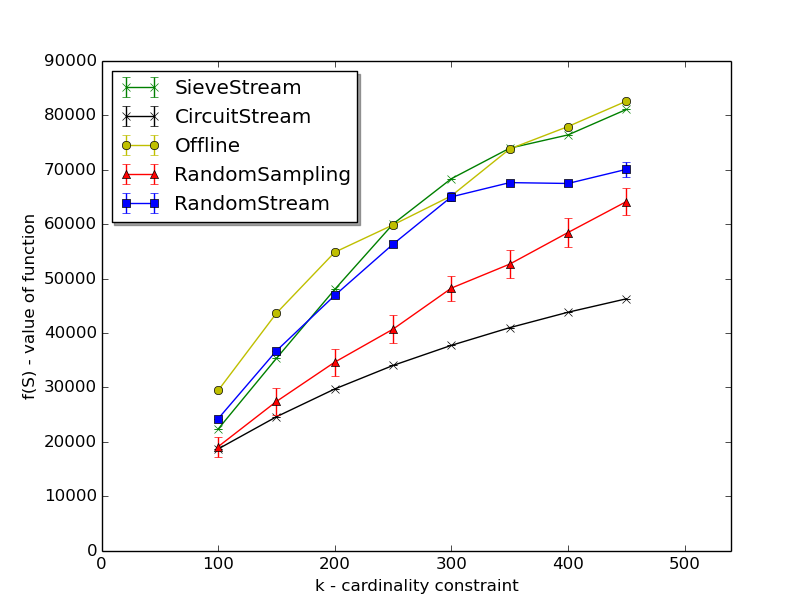
\includegraphics[width=0.5\textwidth]{figures/streaming}\label{fig:streaming-not-shuffle}}    
     \caption{Streaming Algorithms on {\sc Facebook};  $\eps$ is set to be $0.2$ for both \sieveStream and \randomStream; $\gamma$ is set to be $1.0$ for \circuitStream.}
     \label{fig:streaming-facebook}
\end{figure*}



% \begin{figure}[h!]
%     \centering
%     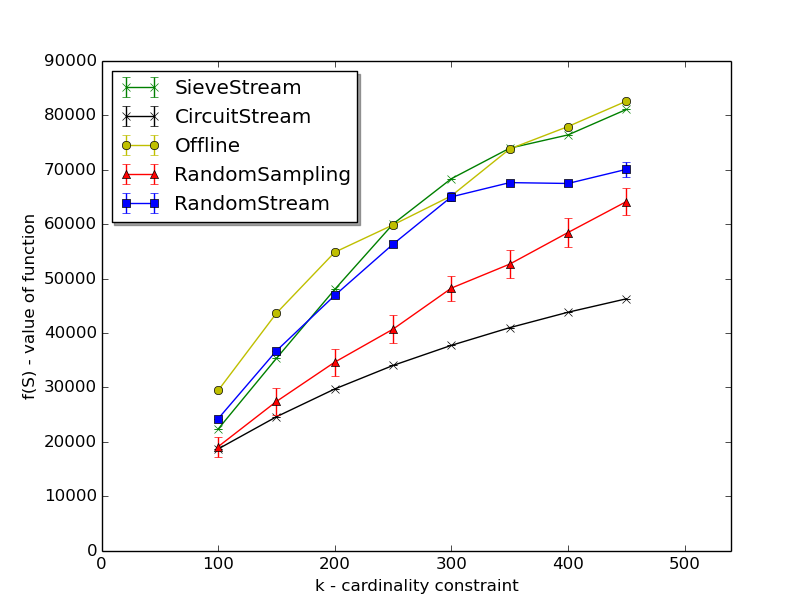
\includegraphics[width=1.1\textwidth]{figures/streaming.png}
%     \caption{{\sc Facebook}: quality of returned solutions, input data is not shuffled; $\eps$ is set to be $0.2$ for both \sieveStream and \randomStream; $\gamma$ is set to be $1.0$ for \circuitStream. }
%     \label{fig:streaming}
% \end{figure}

% \begin{figure}[h!]
%     \centering
%     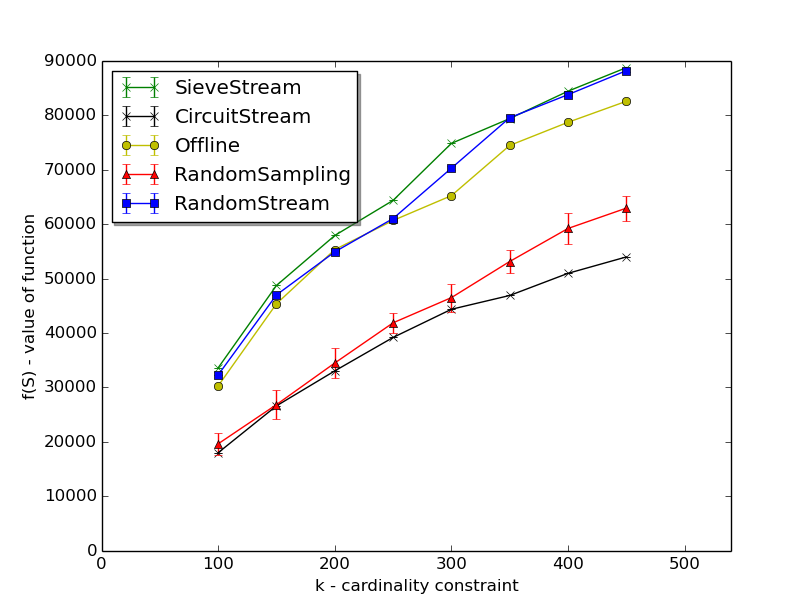
\includegraphics[width=1.1\textwidth]{figures/streaming-shuffle.png}
%     \caption{Quality of returned solutions, input data is shuffled.}
%     \label{fig:streaming-shuffle}
% \end{figure} 




\section{Distributed Submodular Maximization}
\label{sec:distributed}
In this section we mainly focus on testing {\sc GreeDi}-based but omit the algorithms in Kumar et al.\ \cite{KMV+15}. Here are several reasons 1). Kumar et al.\ \cite{KMV+15} has already been experimentally studied and it requires more rounds than {\sc GreeDi}-based algorithms; 2). the implementation of algorithms in \cite{KMV+15} is quite involved and one has to tune many parameters to make it work well. Comparing this algorithm  with others can therefore be difficult;  3) on the other hand, {\sc GreeDi}-based algorithms has less experimental studies but more theoretical results. It would be interesting to conduct experiments to verify those theories.

\subsection{{\sc GreeDI}-based Algorithms}
We described here the general framework of {\sc GreeDi}-based Algorithms. Let $V$ be the ground set we consider; $m$ is the number of machines and $C \in \bbZ^+$ is an parameter; also let $k$ be the cardinality constraint. The algorithm goes as follows:
\begin{itemize}
\item Randomly assign each $v$ to $C$ out of $m$ machines, we obtain subsets $V_1, \ldots, V_m$; each is $\subseteq  V$.
\item Let $\alg$ be an offline algorithm for submodular maximization, $k'$ be a cardinality constraint (it can be different from $k$). Run $\alg$ on each $V_i$ with constraint $k'$, we obtains $U_1, U_2, \ldots, U_m$ as results.
\item Let $U = \cup_i S_i$, run $\alg$ on $U$ with parameter $k$, we obtain $S$ as the result. Also run $\alg$ on $U_1, \ldots, U_m$ with parameter $k$ to obtain $S_1, S_2, \ldots, S_m$.
\item Return the best (i.e. with largest function value) solution among $S$, $S_1, \ldots, S_m$.
\end{itemize}

In our experiment, we use \greedyLazy as \alg. It would  be interesting to see how $k', C$ will affect the quality of the returned results.

\subsection{Experimental Results}
Mirrokni et al.\ \cite{MZ15} argued that when $k'$ and $C$ are increased, the approximation ratio of the {\sc GreeDi}-Based algorithms may slightly increase (however, only slightly above $1/2$). From Figure \ref{fig:distributed-facebook} and Figure \ref{fig:distributed-accidents}, we conclude that those minor theoretical improvement may be less important in practice. In fact, positive correlation between $k'$, $C$ and the approximation is not observed.  
\begin{figure*}[h!]
     \centering
     \subfloat[][Different multiplicity $C$; set $k' = k$; number of machines is $50$.]{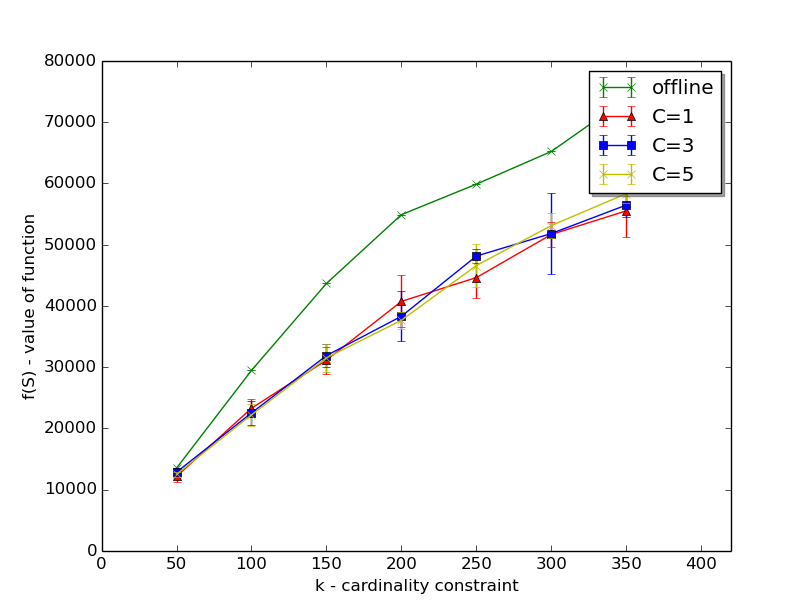
\includegraphics[width=0.5\textwidth]{figures/C}\label{fig:dist-C}}
     ~~
     \subfloat[][Different $k'$; $C$ is set to be $1$; number of machines is set to be $50$.]{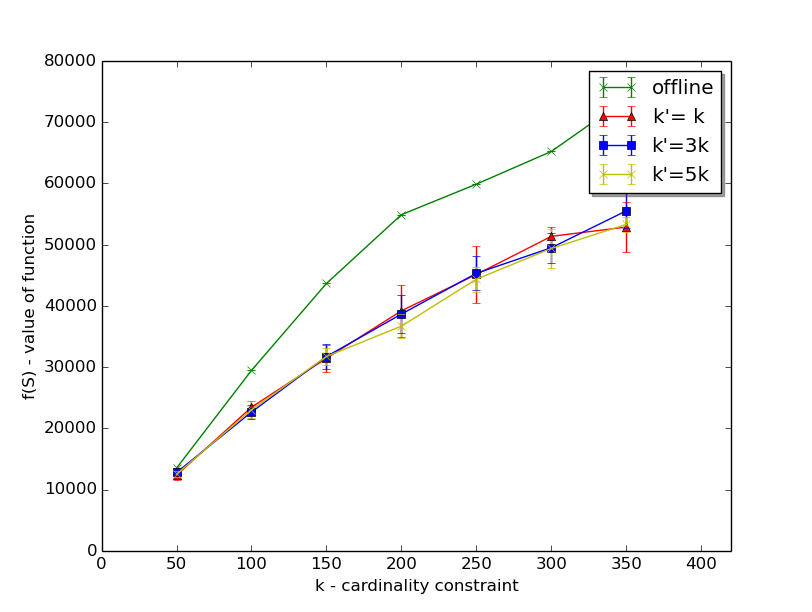
\includegraphics[width=0.5\textwidth]{figures/kk}\label{fig:dist-kk}}    
     \caption{{\sc GreeDi}-based Algorithms on {\sc Facebook} dataset.}
     \label{fig:distributed-facebook}
\end{figure*}


\begin{figure*}[h!]
     \centering
     \subfloat[][Different multiplicity $C$; set $k' = k$; number of machines is $20$.]{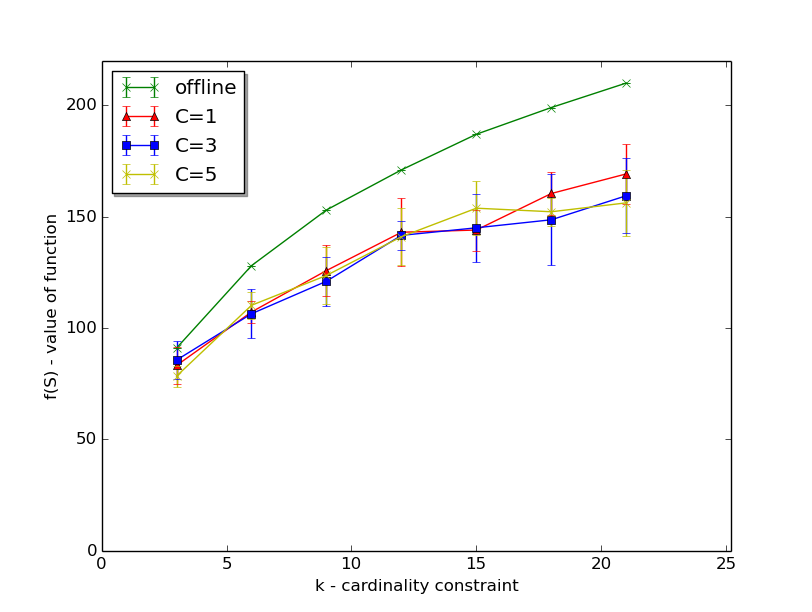
\includegraphics[width=0.5\textwidth]{figures/C-acc}\label{fig:dist-C-acc}}
     ~~
     \subfloat[][Different $k'$; $C$ is set to be $1$; number of machines is set to be $20$.]{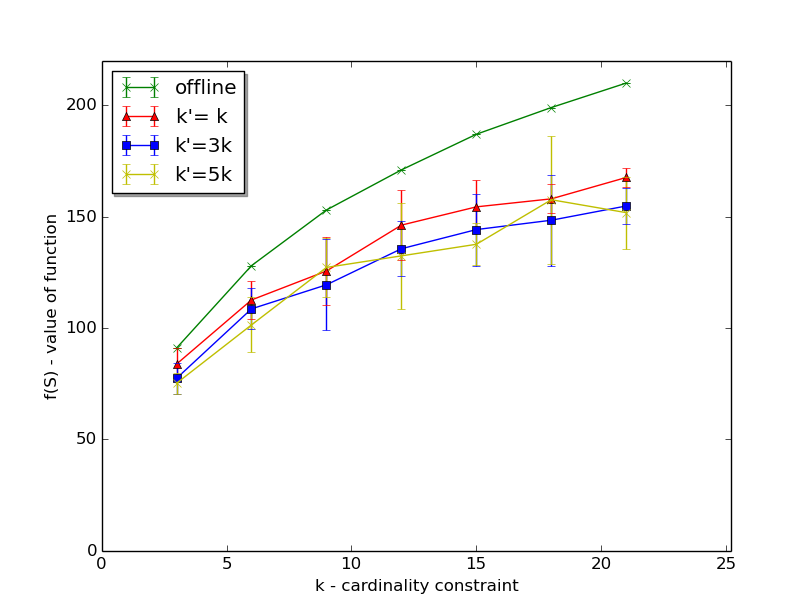
\includegraphics[width=0.5\textwidth]{figures/kk-acc}\label{fig:dist-kk-acc}}    
     \caption{{\sc GreeDi}-based Algorithms on {\sc Accidents} dataset.}
     \label{fig:distributed-accidents}
\end{figure*}



% \begin{figure}[h!]
%     \centering
%     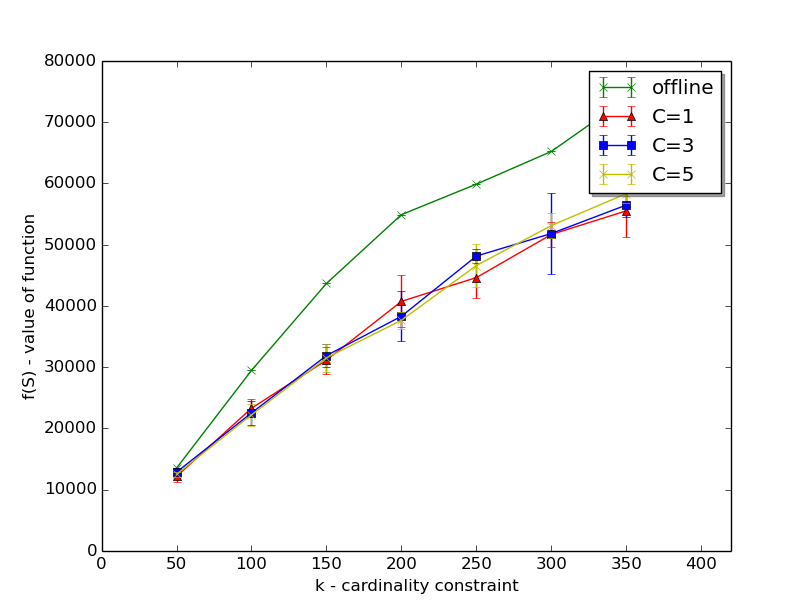
\includegraphics[width=0.5\textwidth]{figures/C.png}
%     \caption{{\sc Facebook}: quality of returned solutions for different multiplicity $C$; number of machines is set to be $50$; $k'$ and $k$ are set to be the same.}
%     \label{fig:dist-C}
% \end{figure}

% \begin{figure}[h!]
%     \centering
%     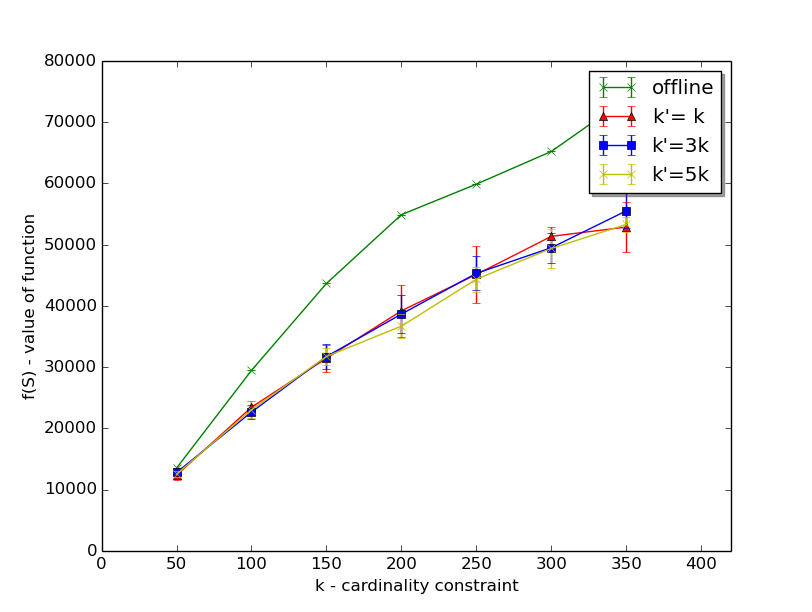
\includegraphics[width=0.5\textwidth]{figures/kk.png}
%     \caption{{\sc Facebook}: quality of returned solutions for different $k'$; number of machine is set to be $50$; the multiplicity $C$ is set to be $1$.}
%     \label{fig:dist-kk}
% \end{figure}


\section{Conclusion}
\label{sec:conclude}
We implemented and tested several algorithms for submodular maximization. In particular, we focus on monotone submodular maximization subject to cardinality constraint, which is the case in most applications we have seen in our survey. Many of the algorithms included in this report are the first time being implemented, and some interesting phenomenons have been observed: e.g. when input data is shuffled, streaming algorithms may give solutions with better quality than the offline greedy algorithm, or increasing $k$ and $C$ actually does not help too much in increasing the approximation ratio.  Due to lack of computation resources, our experiments were simulated in a laptop instead of a cluster. More datasets are necessary to obtain  convincing conclusions. We leave this to future work, possibly a research paper that experimentally evaluates algorithms for streaming/distributed submodular maximization.


%----------- end -------------------------













\bibliographystyle{abbrv}
\bibliography{survey.bib}

%\newpage

%\appendix
%\input{appendix}


\end{document}
